\ifnotes
\else
  \PassOptionsToClass{handout}{beamer}
\fi

\documentclass[10pt,t,svgnames]{beamer}

\usetheme{metropolis} % use metropolis theme

\usepackage{../solarized}         % use solarized themed listings
\usepackage{../stack}             % use the tikzstack environment
\usepackage{appendixnumberbeamer} % do not number appendix frames
\usepackage[scale=3]{ccicons}     % creative commons icons

% fix-up the handling of the notes pages
\ifnotes
  \hypersetup{final}
  \usepackage{pgfpages}
  \setbeamertemplate{note page}[plain]
  \setbeameroption{show notes on second screen=right}
  \AtBeginNote{%
    \let\enumerate\itemize%
    \let\endenumerate\enditemize%
  }
\fi

% overrides default description environment
\newlength\wideleftmargin{}
\newlength\tightleftmargin{}
\newlength\diffleftmargin{}
\setlength\wideleftmargin{6em}    % controls location of term (> is more left)
\setlength\tightleftmargin{1.5em} % controls location of description (same)
\setlength\diffleftmargin{\dimexpr\wideleftmargin-\tightleftmargin}
\makeatletter
\providecommand{\nextline}{
  \setlength\labelwidth{\tightleftmargin}
  \setlength\leftmargin{\tightleftmargin}
  \advance\linewidth\diffleftmargin{}
  \advance\@totalleftmargin-\diffleftmargin{}
  \parshape\@ne\@totalleftmargin\linewidth{}
  \setlength\itemsep{1.5ex}
}
\makeatother
\let\origdescription\description
\let\endorigdescription\enddescription
\renewenvironment{description}{\origdescription\nextline}{\endorigdescription}

%-------------------------------------------------------------------------------

\usepackage{tabularx} % tables

\title{Computer systems}
\date{}
\author{}
\institute{College of Saint Benedict \& Saint John's University}
\begin{document}
  \maketitle

  \begin{frame}[c]{great insights of computer science\footnotemark}
  %{{{1
    \begin{description}
      \item[Bacon, Leibniz, Boole, Turing, Shannon, \& Morse] \hfill \\
        There are only \textbf{two nouns} that a computer has to deal with in
        order to represent ``anything'': 0, 1.
    \end{description}

    \note[item]{``anything'': there are some things computers cannot do --- like
      determine if a program will ever finish.}

    \footnotetext[1]{\href{https://en.wikipedia.org/wiki/Computer\_science\#The\_great\_insights\_of\_computer\_science}{The great insights of computer science}~/~\href{http://creativecommons.org/licenses/by-sa/3.0}{CC~BY-SA~3.0}}
  %}}}1
  \end{frame}

  \begin{frame}[c]{great insights of computer science, cont'd}
  %{{{1
    \begin{description}
      \item[Turing] \hfill \\
        There are only \textbf{five verbs} that a computer has to perform in
        order to do ``anything'':
        \begin{enumerate}
          \item move left one location;
          \item move right one location;
          \item read symbol at current location;
          \item print 0 at current location;
          \item print 1 at current location.
        \end{enumerate}
    \end{description}
  %}}}1
  \end{frame}

  \begin{frame}[c]{great insights of computer science, cont'd}
  %{{{1
    \begin{description}
      \item[Boehm and Jacopini] \hfill \\
        There are only \textbf{three grammar rules} needed to combine these
        verbs (into more complex ones) that are needed in order for a computer
        to do "anything":
        \begin{enumerate}
          \item \emph{sequence}: first do this, then do that;
          \item \emph{selection}: IF such-and-such is the case, THEN do this,
            ELSE do that;
          \item \emph{repetition}: WHILE such-and-such is the case DO this.
        \end{enumerate}
    \end{description}
  %}}}1
  \end{frame}

  \begin{frame}[fragile]{a simple language}
  %{{{1
    \begin{enumerate}
      \item two nouns
      \item five verbs
      \item three grammar rules
    \end{enumerate}
    \vspace{\baselineskip}

    \begin{tabular}{l|l}
      \hline
      \texttt{\textless}    & move left one location\\
      \texttt{\textgreater} & move right one location\\
      \texttt{0}            & print \texttt{0} at current location\\
      \texttt{1}            & print \texttt{1} at current location\\
      \texttt{[}            & if current location is \texttt{0}, then go to
                              instruction after matching \texttt{]}\\
      \texttt{]}            & go to matching \texttt{[} instruction\\
      \hline
    \end{tabular}

    \begin{termblock}
    1>1>0>1>0<<<<[0>]1
    \end{termblock}

    \note[item]{\emph{sequence}: start at left-most instruction and progress a
      single instruction to the right}
    \note[item]{\emph{selection} and \emph{repetition:}
      \texttt{[}\dots\texttt{]} provide both --- repetition is just fancy
      selection}
  %}}}1
  \end{frame}

  \begin{frame}[fragile]{a simple language, cont'd}
  %{{{1
    \vspace{.5\baselineskip}

    \begin{tabular}{l|l}
      \hline
      \texttt{\textless}    & move left one location\\
      \texttt{\textgreater} & move right one location\\
      \texttt{0}            & print \texttt{0} at current location\\
      \texttt{1}            & print \texttt{1} at current location\\
      \texttt{[}            & if current location is \texttt{0}, then go to
                              instruction after matching \texttt{]}\\
      \texttt{]}            & go to matching \texttt{[} instruction\\
      \texttt{\string^}     & add one to the 4-bit number ending at the current
                              location\\
      \hline
    \end{tabular}
    \\[.25\baselineskip]
    \scriptsize{\texttt{\string^} replaces the sequence \texttt{>0<<<<[0>]1}}
    \normalsize

    \begin{termblock}
    1>1>0>1^
    \end{termblock}

    \note[item]{let's add another instruction to increment a number by one}
    \note[item]{we have introduced some \emph{abstraction}}
  %}}}1
  \end{frame}

  \begin{frame}[fragile]{abstraction}
  %{{{1
    \begin{description}
      \item [abstraction] \hfill \\
        A mechanism and practice to reduce and factor out details so that one
        can focus on a few concepts at a time. \\[.5\baselineskip]
        \emph{Abstraction allows program designers to separate categories and
        concepts related to computing problems from specific instances of
        implementation.}\footnote{\href{https://en.wikipedia.org/wiki/Abstraction\#In\_computer\_science}{Abstraction}~/~\href{http://creativecommons.org/licenses/by-sa/3.0}{CC~BY-SA~3.0}}
    \end{description}
  %}}}1
  \end{frame}

  \begin{frame}[fragile]{types of abstraction}
  %{{{1
    \begin{description}
      \item [data abstraction] \hfill \\
        The separation of a data type’s logical properties from its concrete
        implementation. \\[.5\baselineskip]
        In fact, a data type is a data abstraction.
        \begin{termblock}
    boolean found := false
        \end{termblock}
      \item [control abstraction] \hfill \\
        The separation of the behavior of a set of actions from its concrete
        implementation. \\[.5\baselineskip]
        One of the main purposes of programming languages. \\[.5\baselineskip]
        \begin{termblock}
    a := (2 + 3) / 4
        \end{termblock}
    \end{description}

    \note{
      \begin{itemize}
        \item Data abstraction --- take 8 bits, how do you know how to interpret
          the 8 bits? You will need to know if it is an: integer, a
          floating-point value, or something else\dots all three are
          abstractions of the bits
        \item Here is an example --- How is an 32-bit number actually stored in
          our machine? $0x0000010F=271$
      \end{itemize}
      \begin{itemize}
        \item In the example code, \texttt{:=}, \texttt{+}, and \texttt{/} are
          all examples of control abstraction
        \item What vale does \texttt{a} hold?
          \begin{itemize}
            \item You will need to now what data abstraction we are using for
              the numbers \texttt{2}, \texttt{3}, and \texttt{4}, so that you
              know their logical properties, like how addition and division of
              two of them works
          \end{itemize}
        \item Other examples include decisions, iterations, functions
      \end{itemize}
      \begin{itemize}
        \item Where do classes in Java fit?
      \end{itemize}
    }
  %}}}1
  \end{frame}

  \begin{frame}{abstraction levels}
  %{{{1
    \vspace{3ex}
    \begin{columns}
      \begin{column}{.34\textwidth}
        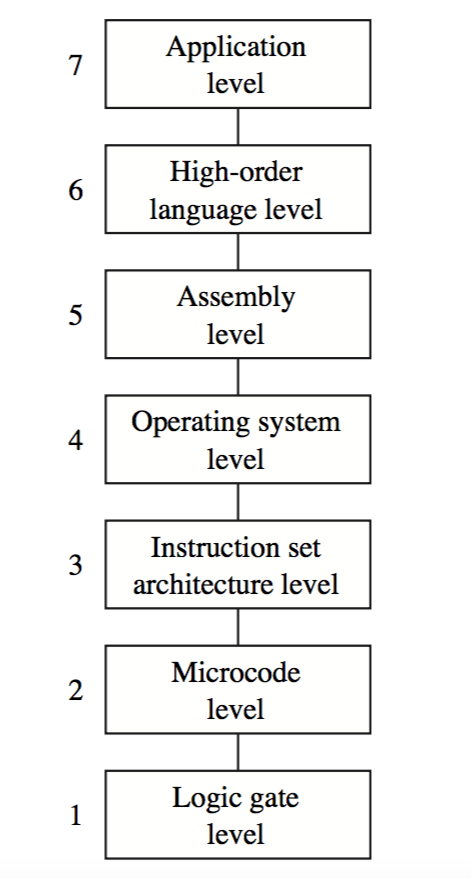
\includegraphics[width=\textwidth]{levels.png}\\
        \hfill \tiny{\href{http://computersystemsbook.com/resources}{Figure P.1}}
      \end{column}
    \end{columns}
  %}}}1
  \end{frame}

  \begin{frame}{history of abstraction}
  %{{{1
    \vspace{3ex}
    \begin{columns}
      \begin{column}{.82\textwidth}
        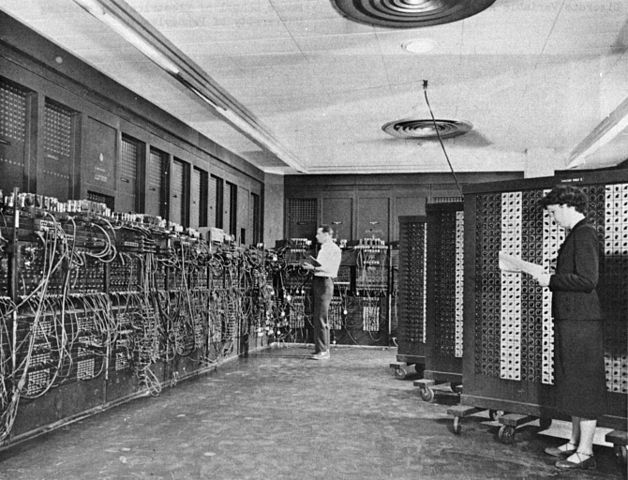
\includegraphics[width=\textwidth]{Eniac.jpg}\\
        \hfill
        \tiny{\href{https://commons.wikimedia.org/w/index.php?curid=55124}{U.S.~Army~Photo}~/~Public~Domain}
      \end{column}
    \end{columns}

    \note[item]{Circa 1946 --- World War II}
    \note[item]{LG1 \& ISA3}
    \note[item]{Six women: Kay McNulty, Marlyn Wescoff, Ruth Lichterman, Betty
      Jean Jennings, and Fran Bilas, programmed the first large-scale general
      purpose machine, ENIAC, to compute ballistics trajectories. Programming
      was done by reorganizing wiring of plugboards.}
  %}}}1
  \end{frame}

  \begin{frame}{history of abstraction, cont'd}
  %{{{1
    \vspace{3ex}
    \begin{columns}
      \begin{column}{.82\textwidth}
        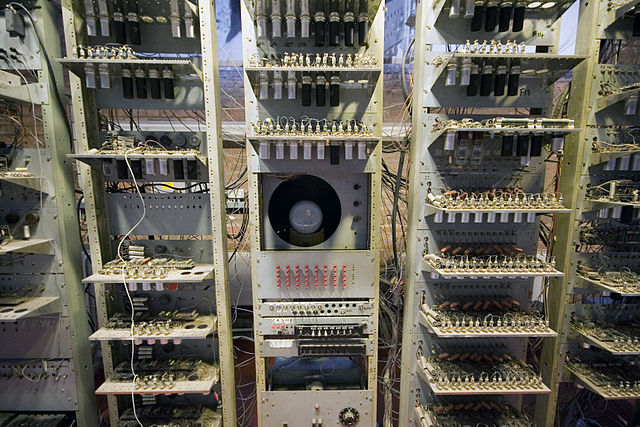
\includegraphics[width=\textwidth]{SSEM.jpg}\\
        \hfill
        \tiny{\href{https://commons.wikimedia.org/w/index.php?curid=55124}{SSEM
        Manchester museum close up}~/~\href{http://creativecommons.org/licenses/by-sa/3.0}{CC~BY~3.0}}
      \end{column}
    \end{columns}

    \note[item]{Circa 1948}
    \note[item]{LG1 \& ISA3}
    \note[item]{Stored program in memory. Programs were entered in binary form
      by stepping through each word of memory in turn, and using a set of 32
      switches known as the input device to set the value of each bit of each
      word to either 0 or 1.}
  %}}}1
  \end{frame}

  \begin{frame}{history of abstraction, cont'd}
  %{{{1
    \vspace{3ex}
    \begin{columns}
      \begin{column}{.52\textwidth}
        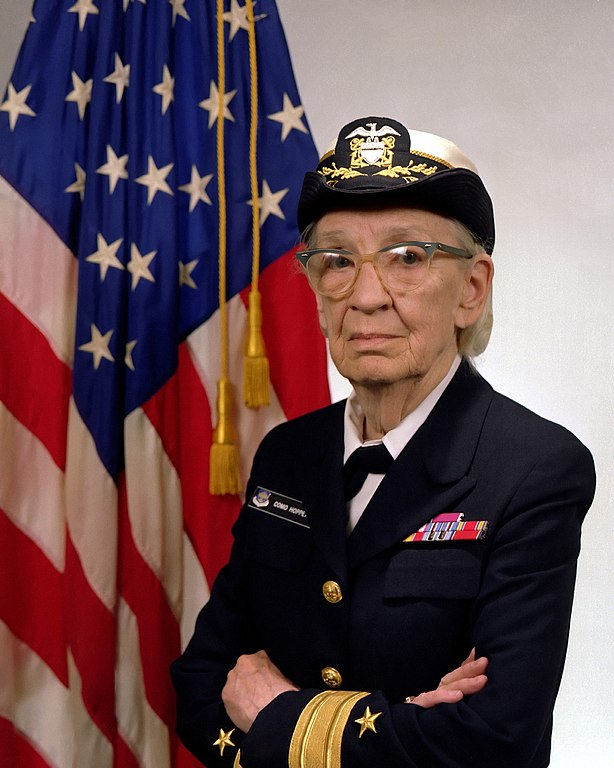
\includegraphics[width=\textwidth]{Grace_Hopper.jpg}\\
        \hfill
        \tiny{\href{https://en.wikipedia.org/wiki/File:Commodore\_Grace\_M.\_Hopper,\_USN\_(covered).jpg}{Commodore~Grace~M.~Hopper,~USN}~/~Public~Domain}
      \end{column}
    \end{columns}


    \note{
      \begin{itemize}
        \item Circa 1951
        \item ASM5 \& HOL6
        \item assembly and high-order languages were developed around the same
          time
        \item Assembly programs are machine-specific, 1-to-1 mapping between
          assembly instructions and machine instructions
        \item some early programming languages still in use today:
          \begin{itemize}
            \item FORTRAN (1954)
            \item LISP (1958)
            \item COBOL (1959)
            \item ALGOL (1958)
          \end{itemize}
      \end{itemize}
    }
  %}}}1
  \end{frame}

  \begin{frame}{history of abstraction, cont'd}
  %{{{1
    %\vspace{3ex}
    %\begin{columns}
    %  \begin{column}{.52\textwidth}
    %    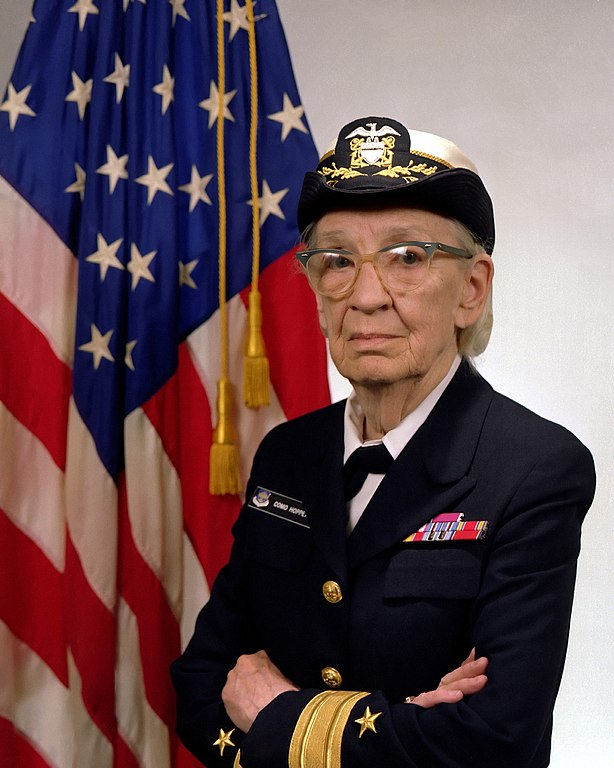
\includegraphics[width=\textwidth]{Grace_Hopper.jpg}\\
    %    \hfill
    %    \tiny{\href{https://en.wikipedia.org/wiki/File:Commodore\_Grace\_M.\_Hopper,\_USN\_(covered).jpg}{Commodore~Grace~M.~Hopper,~USN}~/~Public~Domain}
    %  \end{column}
    %\end{columns}

    \note{
      \begin{itemize}
        \item Circa 1956
        \item OS4
        \item operating system is a piece of software that runs other pieces of
          software
        \item allow multi-tasking and multi-user environments
        \item gives software an interface to hardware --- it manages hardware
          resources
      \end{itemize}
    }
  %}}}1
  \end{frame}

  \appendix

  \begin{frame}[c]
  %{{{1
    \begin{center}\ccbysa\end{center}

    except where otherwise noted, this worked is licensed under
    \href{http://creativecommons.org/licenses/by-sa/4.0/}{creative commons
    attribution-sharealike 4.0 international license}
  %}}}1
  \end{frame}
\end{document}
